
\documentclass[11pt]{amsbook}

\usepackage{../HBSuerDemir}	
\usepackage{float}
\usepackage{wrapfig}


\begin{document}

% ++++++++++++++++++++++++++++++++++++++
\hPage{b1p2/318}
% ++++++++++++++++++++++++++++++++++++++


\begin{wrapfigure}{r}{0.45\textwidth}
	\vspace{-20pt}
	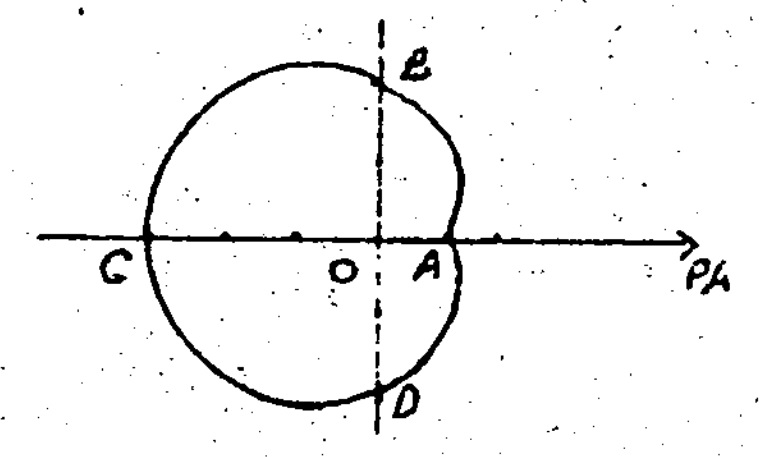
\includegraphics[width=0.8\linewidth]{images/b1p2-318-fig01}
	\vspace{-80pt}
\end{wrapfigure}

Intercepts:
\begin{tabbing}
	$A(0,~1),$\quad \quad      \=     $B(\frac{\pi}{2},~2)$\\
	$C(\pi,~3),$     \>     $ D(-\frac{\pi}{2},~2)$\\ 
\end{tabbing}

\underline{Curves of CASSINl}\par
A curve of CASSINI is the locus of points P whose product of distances from two distinct points $F_{1}, F_{2}$ is constant. $F_{1}, F_{2}$ are said to be the $foci$ of the curve.\par
The equation of a curve of CASSINI in bipolar coordinates is $r_{1}r_{2} = l^{2}$, where $r_{1} = |PF_{1}|,\quad r_{2} = |PF_{2}|$\par

\begin{wrapfigure}{r}{0.4\textwidth}
	\vspace{-25pt}
	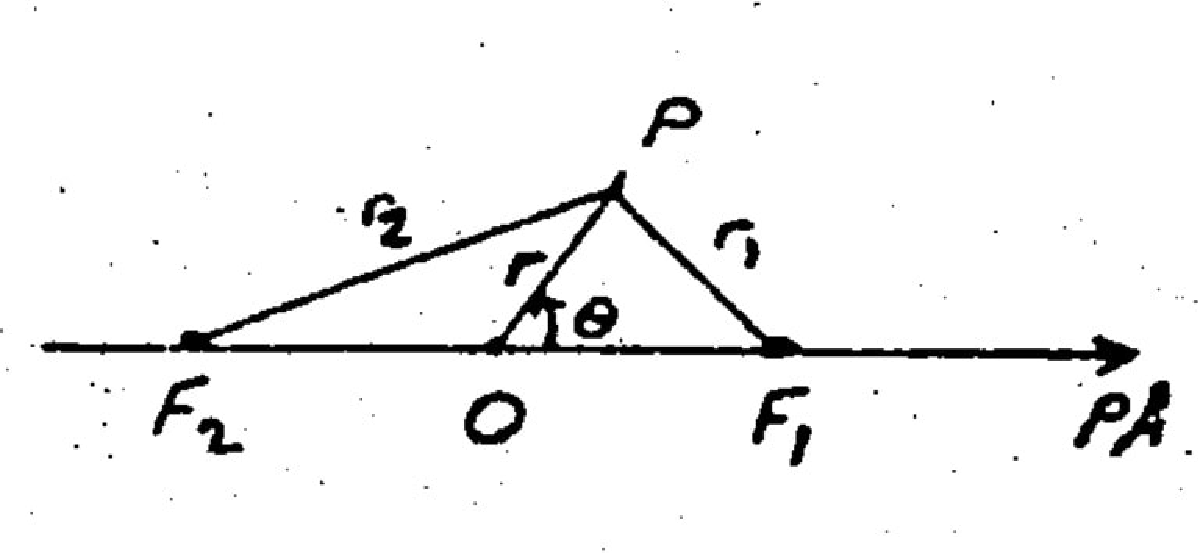
\includegraphics[width=0.9\linewidth]{images/b1p2-318-fig02}
\end{wrapfigure}

We obtain the polar equation by taking the midpoint 0 of $ \big( F_{1}F_{2} \big) $ as pole and $0F_{1}$ as polar axis, with\par
$c = |0F_{1}|=|0F_{2}|:$
\begin{align}
	\label{eq:b1p2_318_firstEquation}
	{r_{1}}^{2}
	{r_{2}}^{2} 
	= l^{4} \quad 
	&\Rightarrow \quad ({r_{1}}^{2} 
		+ c^{2} 
		- 2cr \cos{\Theta})(r^{2} 
		+ c^{2} 
		+ 2cr \cos{\Theta}) 
		= l^{4}\nonumber \\
	& \Rightarrow \quad (r^{2} 
		+ c^{2})^{2} 
		- 4c^{2}r^{2} {\cos^{2}{\Theta}} 
		- l^{4} 
		= 0 \nonumber \\
	& \Rightarrow \quad r^{4} 
		- 2c^{2}(\cos{2\Theta})r^{2} 
		+ c^{4} 
		- l^{4} 
		= 0.
\end{align}

\underline{Case 1. $ l=c$}: The curve passes through the pole ($r=0$) only when $l=c$ yielding the equation

\begin{align}
	\label{eq:b1p2_318_secondEquation}
	r^{2} 
	=  2c^{2} \cos{2\Theta} 
	\quad \quad or \quad \quad 
	 r^{2} 
	= a^{2} \cos{2\Theta}
\end{align}

and this particular curve is called the $lemniscate$ $of$ $Bernoulli$ or simply $lemniscate$.

\begin{figure}[H]
	\centering
	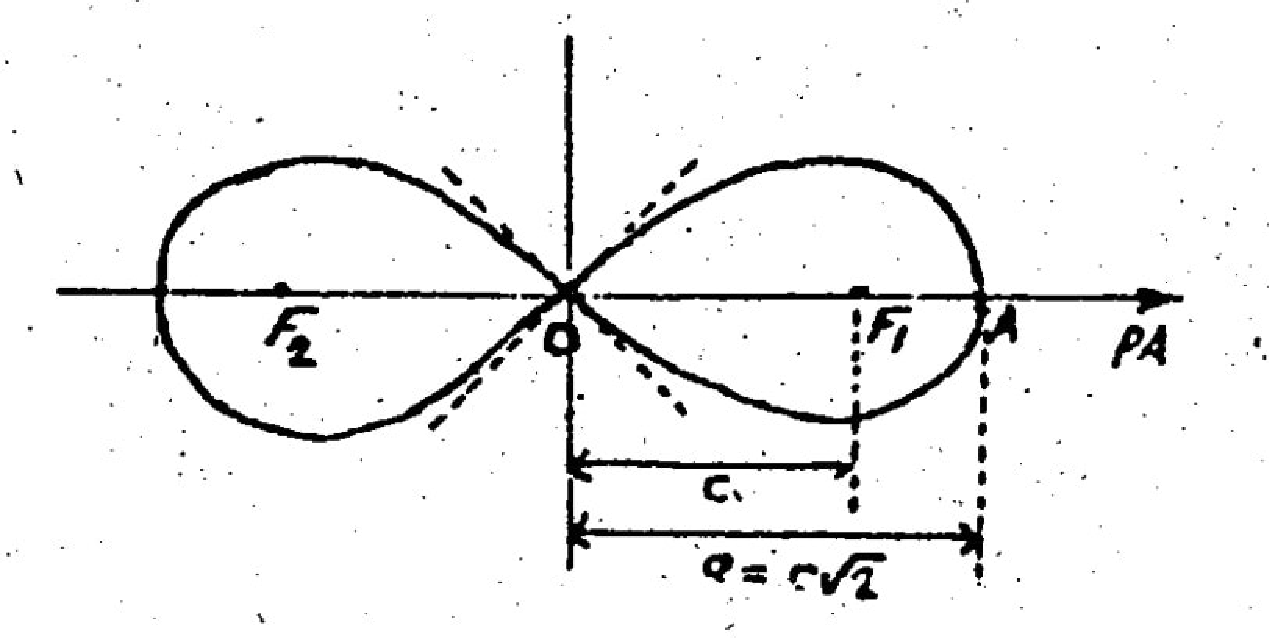
\includegraphics[width=0.45\textwidth]{images/b1p2-318-fig03}
\end{figure}


\footnote{I used wrapfig package to position the image files properly}
\footnote{I used float package to align the third image horizontally center}

\end{document} 